The introduction is split into two sections of background to provide clarity from 1) scientific side - genetics, and 2) mathematics side - Bayesian statistics, described in light of the genetics information.

\section{Genetics}

\subsection{What are Genetic Associations?}
A genetic association is a change in the genetic code that alters the risk of disease. Changes occur in the form of single nucleotide polymorphisms (SNPs), copy number variants (CNV), and indels (micro and microsatellites) 

\subsection{What is GWAS?}
Genome wide association studies identify genetic positions (loci) associated with different disease risks in a population. 

By identifying loci associated with disease either directly find the causal gene or find causal networks that act as signalling pathways, meaning the related gene effects the causal gene. This leads to treatment usage of current or creating candidate therapies. 

\subsection{Important Terms - Genetics}


A \textbf{phenotype} is an expressed trait of interest. This is typically a disease such as cancer or heart disease. In a case-control study, a person with the expressed phenotype of interest is a case, and the person without the expressed phenotype is a control. 

A \textbf{genotype} is the genetic makeup of a organism that will determine its phenotype. The genetic make up is a sequence of base pairs. \texbf{Genotyping analysis} is the process for determining which genetic variants and individual possesses.

A \textbf{single nucleotide polymorphism (SNP)} is a mutation where one base pair is different than the reference genome. Most SNPs are bi-allelic; this makes them easy to be analysed through a binary statistical inferences. 

A \textbf{gene} a stretch of DNA that codes for a particular protein. A \textbf{haplotype} is a group of genes within an organism that was inherited together from a single parent. Haplotypes also refer to the inheritance of clusters of single nucleotide polymorphisms (SNPs), which are variations at single positions in the DNA sequence among individuals [https://www.nature.com/scitable/definition/haplotype-haplotypes-142]. Haplotypes are necessary in creating linkage disequilibrium matrices (discussed below). 

An \textbf{allele} is alternative forms of a gene/trait that are found at the same place on a chromosome. \textbf{Minor Allele Frequency (MAF)} is the frequency (count) at which the second most common allele occurs in a given population. The MAF gives a reference to how common or rare a variant is. A MAF of 0.5 means that the frequency of that specific allele is present in 50 percent of the population.

\texbf{Penetrance}

\subsubsection{Understanding GWAS Manhattan Plot}


\begin{figure}[h]
\centering
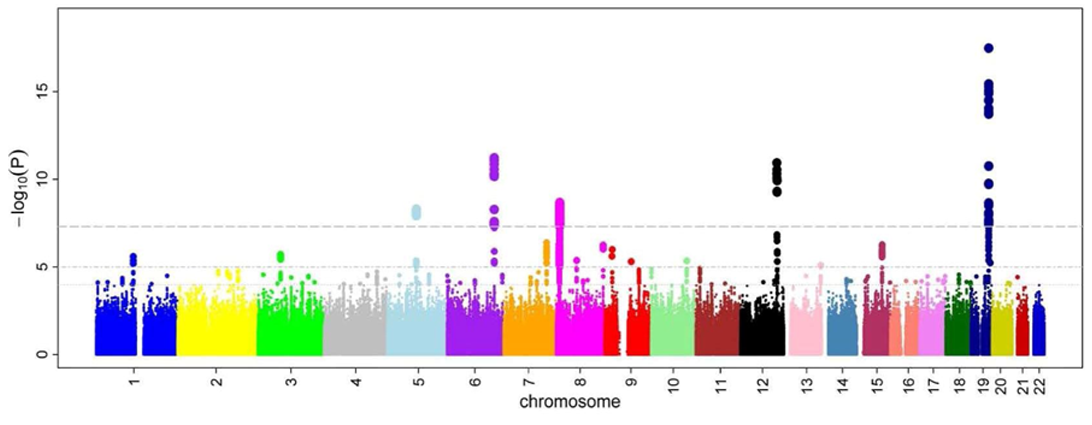
\includegraphics[scale=1.75]{Manhattan_Plot}
\caption{Manhattan Plot}
\label{fig: Manhattan Plot }
\end{figure}

A Manhattan plot (named for it's city skyline like appearance) is used to graphically represent the results of a GWAS. 

Each dot on a Manhattan plot represents one SNP. The x axis is the loci, which is the position of the SNP on the chromosome. On the y axis is the -log(p) of the association of the SNP in the cases compared to the control group. Dots farther up on the y axis represent a SNP that has a stronger association with the phenotype. That is, a genetic mutation associated with disease. The null hypothesis is that each SNP has no association with the phenotype. As stated, GWAS and this analysis identifies candidate genes. In plots where there are multiple highly associated SNPs, this is an indication of pleitropy, which means that the same gene effects more than one phenotype. 

The standard GWAS cutoff of significance used is p$<$5x10\textsuperscript{-8}. In \ref{fig: Manhattan Plot } there are three horizontal dotted lines to represent cutoffs at p$<$5x10\textsuperscript{-4}, p$<$5x10\textsuperscript{-5}, and p$<$5x10\textsuperscript{-8}.  As with other types of studies that have adopted p$<0.05$ as "statistically significant" as a cutoff point, GWAS p-values should also be considered with the issues surrounding this practice. 
GWAS are predicated on the common disease-common variant (CD/CV) hypothesis which states that common disorders are influenced by common genetic variation [@Hemminki2008]. This means the standard GWAS cutoff may not be equipped to handle lower allele frequency spectrum. [@Fadista2016]. Due to limitations and interpretations of frequentist p-values discussed further in \ref{Lead SNP (smallest p-value}, Bayesian methods are used in this study. 

\subsection{What is Linkage Disequilibrium?}

Linkage disequilibrium is the correlation structure that exists among DNA variants in the current human genome as a result of historical evolutionary forces, particularly finite population size (genetic drift), mutation, recombination rate, and natural selection \cite{Visscher2017}. In short, this correlation structure means that SNPs are not statistically independent of each other. LD makes it possible for 80 million SNPs to be arrayed by only 500kb-1Mb SNPs. This is illustrated in \ref{Sample LD Matrix} where a tag SNP that is in high LD can represent a haplotype block and therefore determine other SNPs.  However, LD also makes it difficult to indicate which SNP is causal versus which is a highly correlated neighbouring SNP. 

Because different genes have different recombination probabilities, genetic distance does not equal physical distance. 

LD is expressed by a matrix, where 

[@1000genomeproject]

\subsubsection{Measuring LD}
\paragraph{D'}

\paragraph{r$^2$}

\begin{figure}[H]
\centering
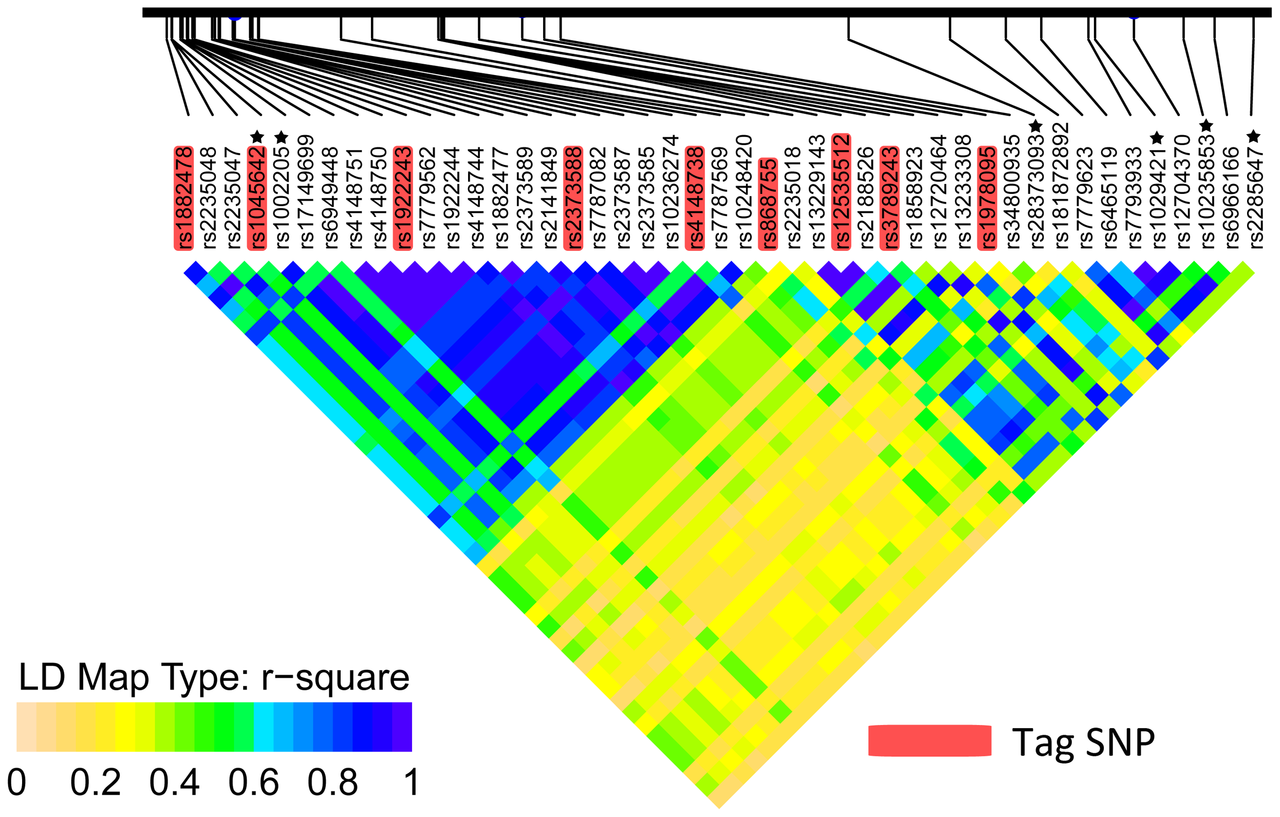
\includegraphics[scale=1.75]{images/LD_matrix.png}
\caption{Example LD Matrix}
\label{Sample LD Matrix}
\end{figure}

\subsubsection{Analysing Manhattan Plot with LD}

In \ref{fig: Manhattan Plot } we see different kinds of patterns of association. In chromosome 5, there are two SNPs above the GWAS cutoff that appear to be "stand alone" or in low LD to the rest of the surrounding SNPs. For this pattern, it is easier to ascertain the causal variant because it is one of the two SNPs. In chromosomes 8, 12, and 19, there are "towers" of SNPs, which means the SNPs are in high LD with each other. This type of patten makes it difficult to ascertain which SNP(s) are the causal variant(s) and which are "noisy neighbours" - SNPs in high LD with causal variant. Chromosome 8 shows an extreme of high LD noise, with a dense tower of SNPs. 

\subsection{Fine Mapping} 
GWAS was the step that \emph{precedes} fine mapping. The goal of GWAS was to find associated genetic changes, while in fine mapping it is to find the causal variant(s). 

Fine mapping is a process in which researchers try and identify the most likely single or set of variants within which the causal variant should be present. The process is done by assigning well-calibrate probabilities of causality to each candidate variant \cite{Spain2015}. 

\subsubsection{Types of Methods in Fine Mapping}

\paragraph{Lead SNP (smallest p-value)} \label{Lead SNP (smallest p-value}
A previous and simple approach was to consider all SNPs of a certain threshold (5 x 10\textsuperscript{-8}) as potential candidates for causality. There are several issues with this, as p-values are influenced by study specific factors such as power (sample size), minor allele frequency, and the effect size (rarely known). Differences in these variables make genetic studies difficult to compare \cite{Spain2015}. 


\paragraph{Lead SNP and LD  "friends" (i.e. r\textsuperscript{2}$>$0.8)}

Another method used was to take the lead SNP, that is the SNP with the highest p-value, and compare it with a certain LD threshold, typically r\textsuperscript{2}	$>$0.8) and consider these neighboring SNPs as the potential causal SNP. This method still ignores properties of the study or locus, as greater power can differentiate SNPs in higher LD. 

\paragraph{Bayesian method}

Association p-values converted to Bayesian posterior probabilities of causality under specific assumptions \cite{Stephens2009} \cite{Wakefield2007}.  These can be summed over sets of variants to generate a posterior probability a causal variant lies in any given set. The posterior probabilities (pp) are the ratio of evidence for each variant being causal versus all the others. This is expressed as $pp/\sum(pp)$. 


\section{Bayesian Statistics}
\subsection{Posterior Probability}
The Bayesian's belief in a binary hypothesis (eg this SNP is causal vs this SNP is not causal) after seeing the data.  Note difference to prior belief.  Bayes Theorem

\begin{equation}
\label{eq-Bayes Theorem}
P(X=x|D)
= \frac{P(X=x) P(D|X=x)}{P(D)}
\end{equation}

\begin{equation}
\label{eq-Bayes Theorem}
{P(X=x|D)}
 = \frac{P(D|X=x) P(X=x)}{\sum(P(D|X=y)(P(X=y))}
\end{equation}

\begin{equation}
\label{eq-Bayes Theorem}
{P(X=x|D)}
 \propto {P(D|X=x) P(X=x)}
\end{equation}

statistical probability that a hypothesis is true, calculated in light of relevant observations. Relevant observations may be defined as both the prior information and the new data that is being analysed, both which together generate the posterior probability. For this reason, the posterior probability is proportionally related to the prior, by the expression of the newly observed data. 

\paragraph{Relationship between p-values and Posterior Probabilities}
The relationship between p-values and posterior probabilities is an inverse relationship. The smaller the p-value which represents the likelihood of observing the data given the null hypothesis, the higher the posterior probability. 

- typically, the SNP is not associated with the 


\subsection{Contrast with Frequentist}

In a frequentist framework a parameter of interest (mean, proportion, rate) is considered fixed and only its estimates vary due to sampling variation. The process of inferring the range of values of  parameter works by considering every possible result that a study could potentially generate. That is, under the same conditions, what would be observed under multiple parallel samples. However this is not possible for many biological phenomena, where a question such as 'What is the probability that a SNP is causal, given the data currently accrued?' [@Kirkwood2005]  

In frequentist statistics the null hypothesis is assumed to be true; that is, it is the starting point of all inference that the observed data is compared to. The p-value reflects the probability of observing data as or more extreme than the data actually observed in the current study, given the null hypothesis \cite{Gurrin2000}. A 95\% confidence interval is interpreted as, if new data were to be repeatedly sampled and analysed, 19 out of 20 intervals would include the true quantity parameter of the being estimated. 

Bayesian statistics incorporate pre-existing information into analyses, in the form of a prior, which is a belief of the distribution of the data before any new data has been observed or incorporated in analysis. This can come a variety of forms such as previous studies, consultation with experts, or theoretical biological models. Under these conditions, spelt out by the Bayes Theorem, a parameter is correctly interpreted as the probability of a hypothesis , given the observed data. 

\subsection{Link with Frequentist}
Here, we discuss the link between a frequentist confidence interval and a Bayesian credible interval with an uninformative prior. When the Bayesian framework is used with an uninformative, the posterior probability is derived from the observed data. The definition of likelihood is bas. An uninformative prior mathematically takes the form of uniform distribution, so that any probability in the distribution has the same proportion. This is similar to frequentist probabilities, which only use the data to estimate the unknown parameter.

\subsection{Important Terms - Statistics}
\paragraph{Credible interval}
A credible interval is a range of values within which an unobserved parameter values falls within a particular subjective probability [Edwards1963]. 

\paragraph{Credible set}
A set of SNPs that contains the causal variant with a pre-specified probability. Each SNP has an assigned prior probability and a posterior probability is calculated, using the likelihood of the data observed [Cite Jenna somewhere here]. The set is determined by a threshold of desired cumulative poster probabilities to reach this cutoff. 

\paragraph{Issues with Credible Sets}
There is currently no explicit quantitative definition for a credible set as there is for a credible interval. A credible assumes a continuous distribution, while a credible set is made up of a discrete distribution for the SNP 

\paragraph{Size of credible set}
For one credible set, the size of the credible set is the belief that the credible set contains the causal variant (eg 90%). 

\paragraph{Coverage of credible set}
If we repeat analysing a list of credible sets, coverage is the amount of times the causal variant is in that credible set. Here coverage can be defined as number of times the causal variant was in the credible set out of the number of simulations run. This can be expressed as a percentage where if 10 credible sets are analysed and 9 of these credible sets include the causal variant, there is 90\% coverage. \emph{Coverage is a frequentist concept because of the nature of repeatability being used to assess Bayesian inferences}. 



\section{Scope of the Study}

This study is done under the one causal variant assumption, meaning there is only one causal variant per credible set. This assumption creates some limitations that are outlined here. 
Colocalization is when a single SNP is associated with multiple phenotypes. Some methods used for colocalization calculate posterior probabilities works by fine mapping each trait under a single causal variant assumption. The two posterior probabilites are then integrated over to calculate probabilities that those variants are shared [@Fortune2018]. Therefore, this analysis may be able to be extended to involve colocalization in the future but is not addressed at this time.  

Copy number variants (CNVs) and variable number tandem repeat (VNTRs) consisting of microsatellites and minisatellites mutations, may account for a 10-15&\% \\ of heritable gene expression variation in humans [@Gymrek2016]. Repetitive DNA is not easily analysed by next generation DNA sequencing methods, which struggle with homopolymeric tracts, that is, parts of the genotype that have the same base pair type repeated many times. Bi-allelic SNPs are not subject to this issue in the way CNVs and VNTRs are, which means they are more easily assayed. This analysis does not address the potential importance of CNVs and VNTRs and assumes that the causal variant can is a bi-allelic SNP. 

Functional annotations are added information known about a SNP in how it effects expressed phenotypes. Functional annotations are typically expressed as coding or non-coding regions of the genes. Among functional annotations are expression quantitative trait loci (eQTL) where a SNP is known to effect a level of expression a particular gene in a particular tissue. Functional annotations are important because physical distance to a gene is not substantive evidence of causality. This means a mutation farther from a gene may play an important role in regulation of that specific gene's expression. 
Although not explored here, methods outlined in this study could be explored by altering the assigned prior value of a SNP in finemap.abf. Reweighting of the posterior probabilities can be done by using fGWAS \cite{Pickrell2014} or PAINTOR methods \cite{Kichaev2014}. 

Different trans-ancestries have different LD patterns. This study does not address any trans-ancestry differences or geographical analysis of subpopulations and their respective potential subtypes.  A SNP that has a small p-value across groups that have different genetic architecture shows a stronger genetic association to a phenotype than if it were present in only one of the groups. In this analysis only one LD matrix is considered at a time, but this could be extended in the future, particularly with relevant open data access from sources such as 1000 Genomes Project. [find spot to cite Jenna's papers here ]. It is important to note that covariates assigned in this study to generate simulations - odds ratios, allele frequencies, and penetrance - can differ in different ancestries. 

\section{Aims}
This study aims to assess Bayesian fine mapping techniques. The study does this by analysing current fine mapping practices and considering how they may be improved. To do this, a metric to capture the amount of disorder in the system - the set of SNPs, was created. Through this method, we are able to say that by making the SNPs with the highest posterior probabilities always incorporated in the credible set through ordering, this contains more information about each SNP. By incorporating the information that SNPs with high posterior probabilities are more likely to be causal, the specified threshold can be reached using a smaller credible set.


\section{Current Practices in Fine Mapping}
Currently it is typical practice that credible sets be ordered by descending posterior probabilities to order the SNP with the highest posterior probability first and the SNP with the lowest posterior probability last. This practice is done because it reduces the credible set, that is the number of candidate SNPs to consider. 

Under this practice, the relationship to size and coverage are considered. 

\subsection{Relationships to Ordering}
\paragraph{Size}
The relationship between ordering and credible set size is an inverse relationship. This is simple to see in an example. Say there are 100 SNPs and the 97th SNP is the causal variant with the lowest p-value, and therefore has the highest posterior probability. An unordered credible set with a pre-specified threshold (cumulative sum of posterior probabilities), would need to take 97 SNPs to achieve the specified threshold. The ordered credible set could achieve the same threshold with many fewer SNPs. This is illustrated below.
\paragraph{Coverage}